\chapter{Outline and Contributions}
In this section, we provide a brief overview of the key contributions presented in this thesis, summarized in Figure \ref{fig:contributions}.
%\gls*{RFF} 

\begin{figure}[h!]
    \centering
    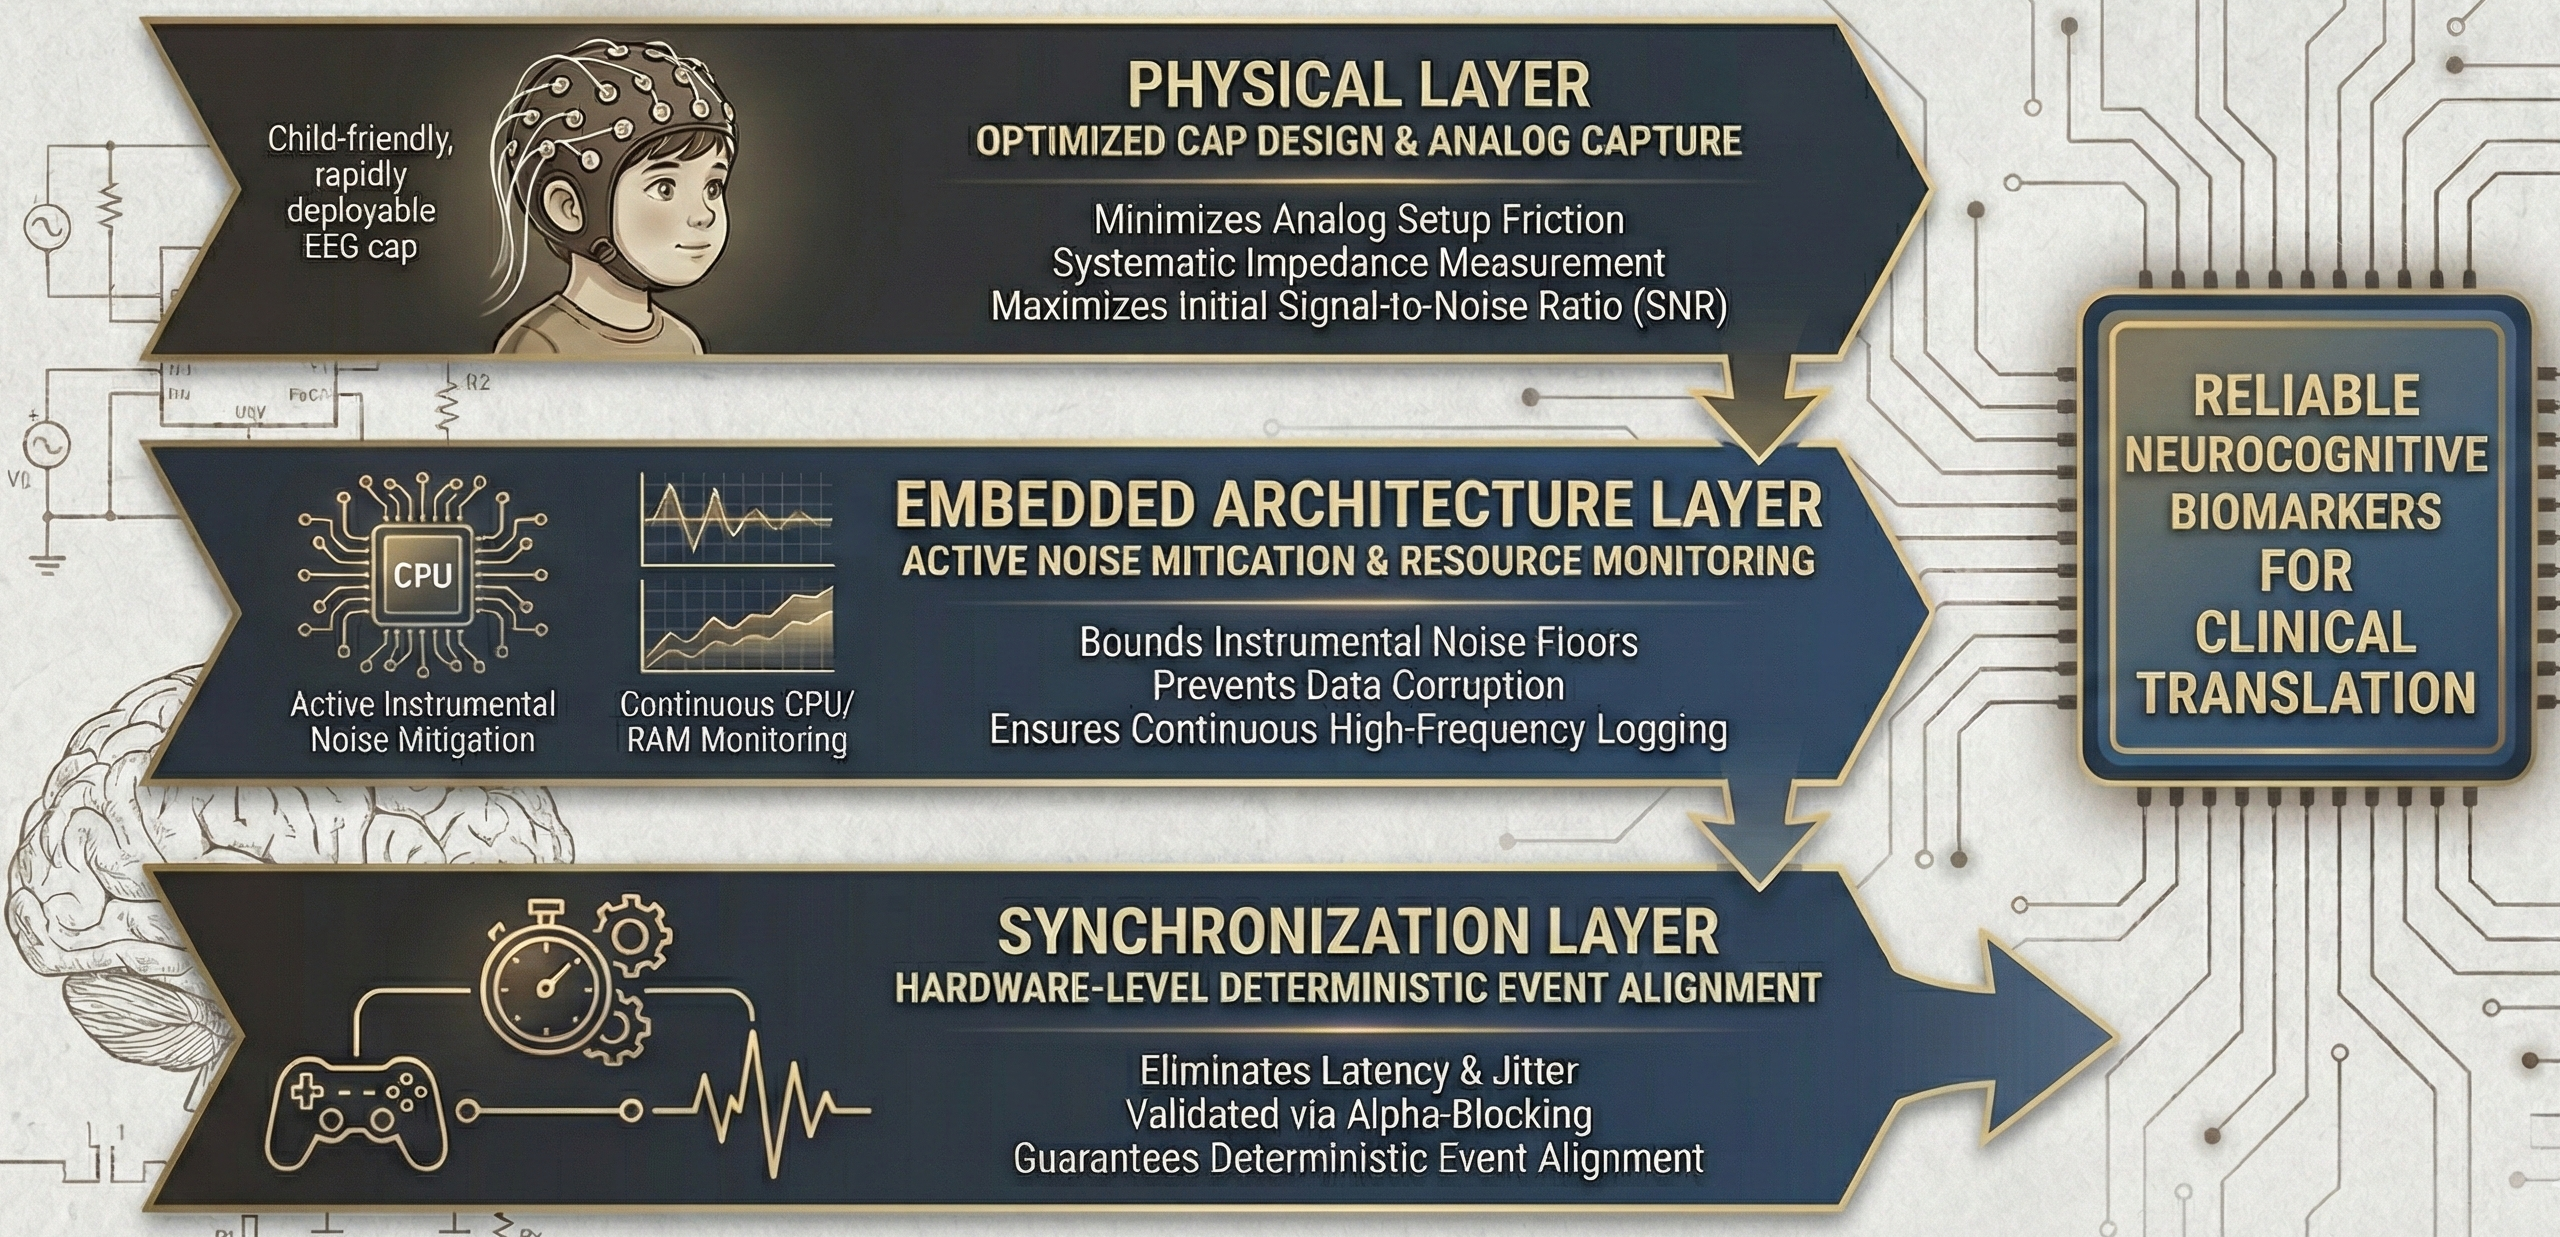
\includegraphics[width=1\linewidth,height=10cm]{Figures/outline_and_contributions/contributions.png}
    \caption[Scheme of an EQA task, illustrating the main contribution of this thesis, which allows finding the most relevant tokens to provide a precise answer to the question asked by the user.}
    \label{fig:contributions}
\end{figure}

This work contributes to the understanding of how transformer architectures work internally in the EQA task, based on the RawAtt \cite{abnar2020quantifying} interpretability technique, which allows finding the most relevant tokens of the context when answering a question made by the user. Our hybrid model represents a significant advance in interpretability by offering a clearer and more consistent interpretation of the results, paving the way for future research in this field.





